%%%%%%%%%%%%%%%%%%%%%%%%%%%%%%%%%%%%%%%%%
% Stylish Article
% LaTeX Template
% Version 2.0 (13/4/14)
%
% This template has been downloaded from:
% http://www.LaTeXTemplates.com
%
% Original author:
% Mathias Legrand (legrand.mathias@gmail.com)
%
% License:
% CC BY-NC-SA 3.0 (http://creativecommons.org/licenses/by-nc-sa/3.0/)
%
%%%%%%%%%%%%%%%%%%%%%%%%%%%%%%%%%%%%%%%%%

%----------------------------------------------------------------------------------------
%	PACKAGES AND OTHER DOCUMENT CONFIGURATIONS
%----------------------------------------------------------------------------------------

\documentclass[fleqn,10pt]{SelfArx} % Document font size and equations flushed left

\usepackage{listings} % Required to insert dummy text. To be removed otherwise
\usepackage[titletoc]{appendix}


%\lstset{numberstyle=\tiny,numbersep=5pt,language=Lisp,
%  stringstyle=\ttfamily\small,basicstyle=\ttfamily\footnotesize,
%  showstringspaces=false,breaklines}

\lstset{
    language=LISP,
    basicstyle=\ttfamily\small,
    showstringspaces=false,
    columns=fixed,
    basewidth=.5em,
    escapeinside={&[}{]&},
    aboveskip=12pt,
    belowskip=12pt,
    lineskip=-1pt,
    frame=none
  }
%----------------------------------------------------------------------------------------
%	COLUMNS
%----------------------------------------------------------------------------------------

\setlength{\columnsep}{0.55cm} % Distance between the two columns of text
\setlength{\fboxrule}{0.75pt} % Width of the border around the abstract

%----------------------------------------------------------------------------------------
%	COLORS
%----------------------------------------------------------------------------------------

\definecolor{color1}{RGB}{0, 0, 0} % Color of the article title and sections
\definecolor{color2}{RGB}{0,20,20} % Color of the boxes behind the abstract and headings

%----------------------------------------------------------------------------------------
%	HYPERLINKS
%----------------------------------------------------------------------------------------

\usepackage{hyperref} % Required for hyperlinks
\hypersetup{hidelinks,colorlinks,breaklinks=true,urlcolor=color2,citecolor=color1,linkcolor=color1,bookmarksopen=false,pdftitle={Title},pdfauthor={Author}}

%----------------------------------------------------------------------------------------
%	ARTICLE INFORMATION
%----------------------------------------------------------------------------------------

\JournalInfo{CS389R Recursion and Induction, UT Austin, 2015} % Journal information
\Archive{Dr. Warren Hunt, T.A. Dr. Nathan Wetzler} % Additional notes (e.g. copyright, DOI, review/research article)

\PaperTitle{ACL2: Modeling Adders (and other circuits)} % Article title

\Authors{Cole Stewart\textsuperscript{1}} % Authors
\affiliation{\textsuperscript{1}\textit{Department of Computer Science, University of Texas at Austin}} % Author affiliation

\Keywords{ACL2 -- Circuits -- Verification -- Modeling} % Keywords - if you don't want any simply remove all the text between the curly brackets
\newcommand{\keywordname}{Keywords} % Defines the keywords heading name

%----------------------------------------------------------------------------------------
%	ABSTRACT
%----------------------------------------------------------------------------------------

\Abstract{Discusses different variations of modeling and verification of simple circuits
in ACL2. In particular, a method of converting a circuit diagram to a verifiable ACL2
model is discussed, and a lookahead adder from the Texas Instruments TTL vol. 3 is modeled
and verified.}

%----------------------------------------------------------------------------------------

\begin{document}

\flushbottom % Makes all text pages the same height

\maketitle % Print the title and abstract box

\tableofcontents % Print the contents section

\thispagestyle{empty} % Removes page numbering from the first page

%----------------------------------------------------------------------------------------
%	ARTICLE CONTENTS
%----------------------------------------------------------------------------------------

\section*{Introduction} % The \section*{} command stops section numbering

\addcontentsline{toc}{section}{Introduction} % Adds this section to the table of contents
Formalization and verification of circuit outputs has been a necessary task since the 
introduction of computing. In the beginning, there were no formal verification tools available 
to automate that process either. ACL2 offers a first-order logic and programming language
where systems can be modeled and verified in an automated way. Circuits, in particular, can 
be modeled and logically represented differently. 
This project aimed to accomplish 3 goals:

\begin{enumerate}
\item Creation of a Java tool for generating ACL2 models from circuits defined in CEDAR Logic Simulator, which we call CircuitToAcl2
\item Use of tool to generate ACL2 models for each module in CEDAR Logic Simulator and verify correctness
\item Prove correctness of carry-lookahead adder as defined by the SN74AS181 and SN74AS182 in the Texas Instruments TTL with the use of binary decision diagrams (BDD), unlabeled binary decision diagrams (UBDD), and different physical model representations
\end{enumerate}

%------------------------------------------------

\section{Generating ACL2 Models}
CEDAR Logic Simulator\cite{cedar} is a software simulator for circuits involving logic gates and other logical modules such as full adders and registers that is often used in teaching computer engineering courses. In the beginning of the project, other tools such as LogiSim were examined as possible arguments to a model conversion application, but no tool seemed to represent the internal graph in a meaningful way as well as CEDAR. All the tools which were examined used XML for output.

Generating ACL2 models from CEDAR Logic Simulator was slightly more difficult than was originally anticipated. The XML which was output by CEDAR was malformed in some sections and had to be preprocessed and modified to be well-formed XML before being fed into the XML parser. Being careful not to integrate the generator with one specific metamodel was also a bit of a challenge. The most difficult part of the process, however, was ensuring a gate never came after another gate which depended on it in the ACL2 let* expression output by the application. Solving this problem involved performing a graph traversal through the circuit starting at the inputs. Performing this traversal also allowed a cycle detection to be performed simultaneously. Although the framework is general enough to support the creation of other models in ACL2, in the end only one model was supported. This model is based on overloading primitive ACL2 functions to serve as logic gates in a circuit. No cycles are allowed in the circuit, as no state is allowed.

\subsection{Warming Up}
\subsubsection{Creating a Model of a 4-bit Comparator}
CEDAR has a library of modules which are essentially small circuits composed of gates which can be connected alongside other gates. One such module in the library was a 4-bit comparator. As a simple example, the comparator was first modeled to get warmed up to the process of defining and verifying correctness of circuits in ACL2. In Figure 1 a screenshot of CEDAR Logic is shown which contains a simple comparator with 3 outputs: $a>b$, $a<b$, and $a=b$. Appendix A shows the output of CircuitToAcl2 with input defined by the circuit in Figure 1.

\begin{figure}[ht!]
  \caption{A 4-bit comparator in CEDAR Logic Simulator}
  {%
\setlength{\fboxsep}{0pt}%
\setlength{\fboxrule}{1pt}%
\fbox{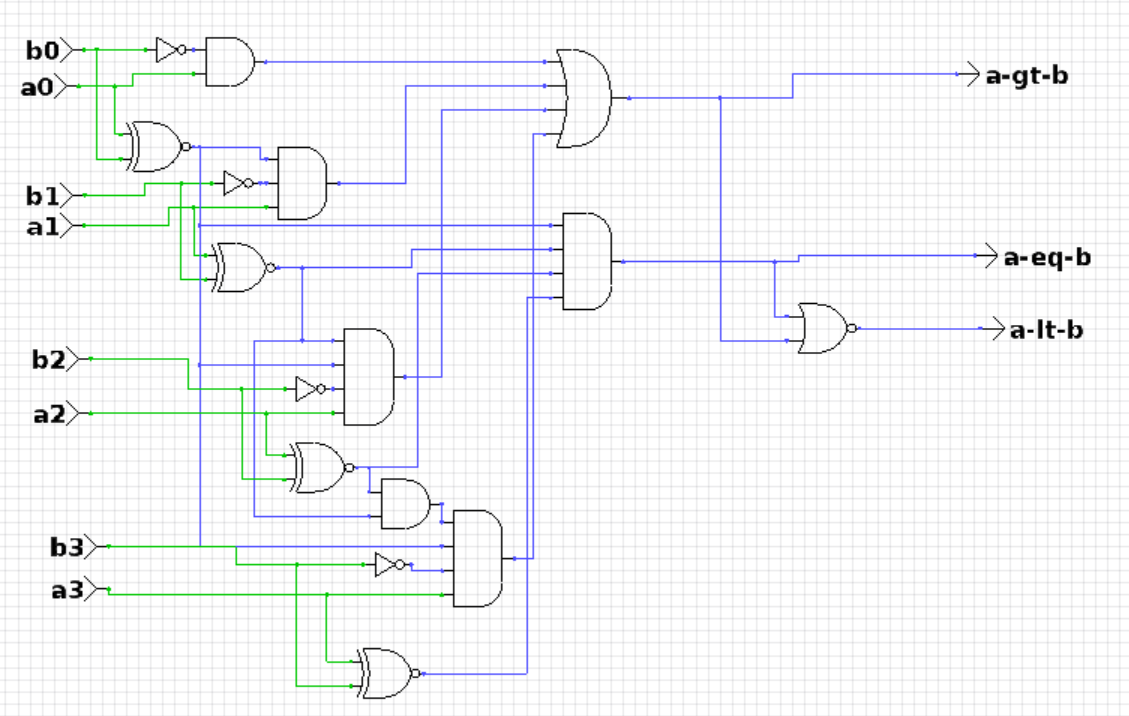
\includegraphics[width=\columnwidth]{comparator.png}}%
}%
\end{figure}

\subsubsection{Defining a Functional Comparator}
In order to prove the correctness of this circuit using ACL2, we first needed to define our own model for the 3 functions of the comparator. Note that these functions, as well as all other functions in this document assume the inputs are in little-endian order. 

\begin{lstlisting}
;; = relation for variable-length vectors 
(defun v-= (a b)
  (if (atom a)
      (atom b)
    (and (xnor (car a) (car b))
         (v-= (cdr a) (cdr b)))))

;; < relation for variable-length vectors
(defun v-< (a b)
  (if (atom a)
      nil
    (if (equal (cdr a) (cdr b))
        (and (not (car a)) (car b))
      (v-< (cdr a) (cdr b)))))

;; > relation for variable-length vectors
(defun v-> (a b)
  (v-< b a))
\end{lstlisting}

After we have defined a functional model that implements the functional output of a comparator, we can then leverage ACL2's reasoning system to check if the created model is correct. We can prove that these functions produce the correct output by converting the input bit vectors into natural numbers. The defthm declaration for the $<$ relation is shown below. The v-to-nat function was provided by Dr. Hunt. It converts a little-endian bit vector represented as a boolean list to a natural unsigned number. The induction hint to use the induct-hint-both function to define the schema of inductive steps simply tells the theorem prover to reduce both a and b to be the 
\lstinline{(cdr a)} and \lstinline{(cdr b)} in the inductive hypothesis. 

\begin{lstlisting}
(defthm v-to-nat-equal
  (implies (and (boolean-listp a)
                (boolean-listp b)
                (= (len a) (len b)))
           (equal (= (v-to-nat a)
                     (v-to-nat b))                   
                  (equal a b)))  
:hints (("Goal" :induct (induct-hint-both a b))))
  
(defthm v->-correct
  (implies (and (boolean-listp a)
                (boolean-listp b)
                (= (len a) (len b)))
           (iff (v-> a b)
                (> (v-to-nat a) (v-to-nat b)))))
\end{lstlisting}

After the previous theorems are verified and entered into the ACL2 logic, we can use them to verify the netlist that was generated from the first step. This accomplished by presenting the theorem prover with an equality relation that involves functions from the general model and the netlist we are trying to verify. 

\begin{lstlisting}
(defthm comparator-netlist-compares-<
  (implies 
    (boolean-listp '(a0 a1 a2 a3 b0 b1 b2 b3))
    (equal (v-< '(a0 a1 a2 a3) '(b0 b1 b2 b3))
           (nth 2 (4-bit-comparator-netlist 
                    a0 a1 a2 a3 b0 b1 b2 b3)))))
\end{lstlisting}

The above statement tells the story for the $<$ relation, as the \lstinline{defthm} statements for the other functions are almost identical. This pattern of explicitly defining the variables to be used in the proof in the hypothesis of the theorem will be carried over to each of the different methods used to prove correctness of these these circuits which have a finite definition.

\begin{figure*}[ht]\centering
\caption{A 64-bit carry lookahead adder from the TTL\cite{TTL}}
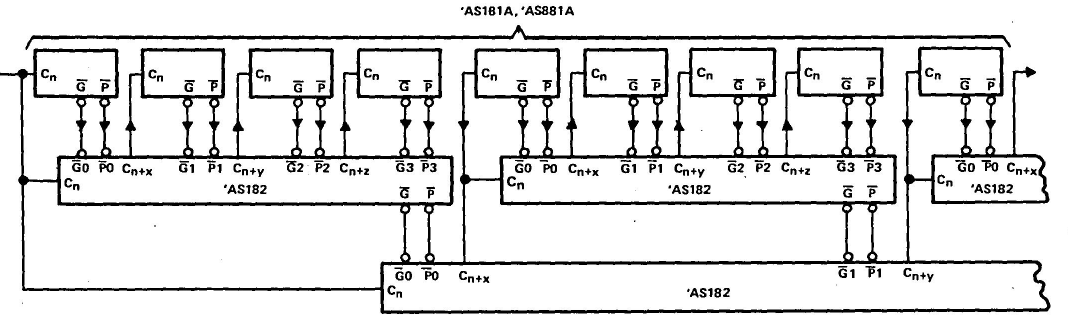
\includegraphics[width=\linewidth]{lookahead.png}
\end{figure*}
\section{The Carry Lookahead Adder}
As a more interesting example, consider a carry-lookahead adder. A carry-lookahead adder is a type of logical adder which computes addition in logarithmic time. In traditional ripple carry adders, each adder must wait for the output carry to be propagated from the previous adder unit, resulting in a computation that is linear in time. Lookahead units compute $N-1$ carry bits based on the values of a propagate and generate bit from each of the $N$ adders that are connected as masters to the lookahead.

The Texas Instruments TTL\cite{TTL} defines two modules which can be used to create such an adder:
\begin{itemize}
\item SN74AS181A -- an ALU circuit with support for addition of two 4-bit vectors
\item SN74AS182 -- a lookahead carry circuit for performing addition in logarithmic time
\end{itemize}

Appendix A contains the gate diagrams for these modules.

\footnote{The arrows connecting the carries from the lookahead in Figure 2 are pointing in the wrong direction. This is a mistake in the TTL.}Figure 2 shows an excerpt of such a system with 16 SN74AS181A modules functioning as adders with 5 SN74AS182 lookahead units.

An interesting property of the lookahead adder exists in the mutual dependency between the lookahead unit and the adders. Appendix A.2 and A.3 show the gate diagram of the '181 and '182 modules. Looking at these diagrams and observing how these modules connect together illustrates that each carry produced by the '182 requires the values for the propagate and generate bits for the previous adders be present, and the adders need the carry produced by the lookahead to perform their logical function. For our simple netlist model, this poses a problem. Since the model of the circuit is embedded into ACL2 logic itself, the ACL2 evaluator has no way of knowing how to split up the complete circuit to complete the computation. There are 2 approaches of solving this problem:
\begin{itemize}
\item Evaluate the '182 module repeatedly, being careful to supply values to unused inputs which will not affect the desired outputs of the module
\item Flatten the circuit, effectively isolating the functionality of each output in the '182
\end{itemize}

There is another way of modeling the circuits which hides these problems associated with evaluation. By representing the model as data instead of ACL2 logic directly, an evaluator can be written which gives functional meaning to the data and provides a nice abstraction to the user. This approach is discussed later.

\subsection{The SN74AS181 from the TTL}
When the '181 is in $add$ mode, it offers 7 inputs and 11 outputs that are relevant for addition. The '181 accepts 2 4-bit input bit-vectors and an input carry. The output consists of an output carry bit, 4 bits comprising the first input vector, 4 bits comprising the second input vector, a propagate bit, and a generate bit. The '181 was already defined by Dr. Hunt, as well as a generic adder for

\subsection{The SN74AS182 from the TTL}
The first order of business was to create a functional model of the F74182 lookahead unit. Defining a model for the SN74AS182 in ACL2 was relatively straightforward. For this step the Java tool was not used to create the netlist in ACL2, however it is important to note that CircuitToAcl2 would produce an equivalent model. In the beginning of the project there was a misconception that creating the models by hand would take more time than first creating a gate-level representation of the circuit in software such as CEDAR. Doing this step by hand pointed out that creating the model is not the most time-consuming step involved in the process of verifying the correctness of a circuit, or any system for that matter. Instead, the difficulty lies in coming to agreement on defining how the models in the system are to be represented so that verification can take place. 

\section{Verifying Correctness of a 16-bit Carry Lookahead Adder Using BDD's}
The first approach used in providing a logical representation for the models in ACL2 involved labeled binary decision diagrams. A binary decision diagram is a method for representing boolean functions that works exceptionally well for verifying hardware descriptions\cite{bdd}. BDD's allow for the internal branching of an acyclic circuit to be represented in a deterministic way, meaning that two circuits defined as a set of finite branching functions can be tested for equivalent functionality when the inputs are boolean values. Labeled BDD's allow us to propose a theorem in ACL2 using boolean variables without explicitly embedding BDD's into the model. Using labeled BDD's, ACL2 will bind the variable names to construct BDD nodes automatically. 

Modeling the lookahead adder in this way allowed the definition of simple boolean functions to model the output functions of the circuit in the same way as the comparator example in Section 1.1. For the '181 3 output groups from the circuit needed a general function in ACL2 which functionally and recursively defined the property a specific output was intended to hold:
\begin{itemize}
\item A function for $N$-bit vector addition
\item A function for producing the propagate bit
\item A function for producing the generate bit
\end{itemize}
Then, for the '182 another 3 functions were needed:
\begin{itemize}
\item A function for producing a carry bit given a propagate and generate vector
\item A function for producing the propagate bit
\item A function for producing the generate bit
\end{itemize}

\subsection{Modeling an Adder with Propagate and Generate}
A generic adder was was already defined by Dr. Hunt, however, it did not define the outputs for the propagate and generate functions of the adder. Modeling the propagate functionality of the '181 is simple, as it is only high when both bits are high at the same index in the two input vectors used in addition. The generate function is a bit trickier though, as the output depends on the result from the output at the previous index. Most of these algorithms involve iterating over the input vectors and observing some function of the input vectors at a specific index. These functions are shown below:

\begin{lstlisting}
(defun v-propagate (a b)
  (if (atom a)
      nil
    (or (and (car a) (car b))
        (v-propagate (cdr a) (cdr b)))))

(defun v-generate-r (a b prev)
  (if (atom a)
      prev
    (v-generate-r (cdr a) (cdr b)
                  (if prev
                      (or (car a) (car b))
                    (and (car a) (car b))))))

(defun v-generate (a b)
  (v-generate-r a b t))
\end{lstlisting}

These functions and a few unwinding theorems for the BDD algorithm were enough to show that these produce the same output as the SN74AS181 when two 4-bit vectors are used as input. When using labeled BDD's, the theorem prover needs a way to open up the function when an input is a consp. As an example, the unwinding theorem for \lstinline{v-propagate} is shown below:
\begin{lstlisting}
(defthm v-propagate-cons
  (equal (v-propagate (cons ai a) (cons bi b))
         (or (and ai bi) (v-propagate a b))))
\end{lstlisting}

\subsection{Modeling the Lookahead's Propagate and Generate Outputs}
Like the '181, the '182 has a propagate and generate output as well so that systems like the 64-bit adder in Figure 2 can be implemented. However, the output of these functions is slightly different than the '181. The lookahead ``propagates`` if any of the input propagate bits are high. This is a simple vector-or function which performs the bitwise-or of every element in the propagate input vector. The lookahead ``generates`` according to a more complex function. By looking at the gate diagram for the SN74AS181 in Appendix A, the function for the generate bit looks like the following:

\begin{lstlisting}
(or (and g0 g1 g2 g3)
    (and p1 g1 g2 g3)
    (and p2 g2 g3)
    (and p3 g3))
\end{lstlisting}

This pattern is recognized by the recursive definition below:

\begin{lstlisting}
(defun v-lkahead-generate-r (p g prev)
  (if (atom p)
      prev 
   (v-lkahead-generate-r (cdr p) (cdr g)
                  (if prev
                      (car g)
                    (and (car p) (car g))))))

(defun v-lkahead-generate (p g)
  (v-lkahead-generate-r p g t)) 
\end{lstlisting}


\subsection{Modeling the Lookahead's Carry Outputs}
Modeling the carry outputs of the lookahead was similar to the process of modeling the generate bits for the '181, with the major exception that the lookahead has multiple carry outputs. We have to define the recursive pattern not only in composing the result of one of the carry outputs, but also define the pattern that produces a vector of carry outputs. Observe the functional values for the 3 carries from the lookahead module:

\begin{lstlisting}
;; cn+x 
(nor (and p0 g0)
     (and cin g0))

;; cn+z
(nor (and p1 g1)
     (and p0 g0 g1)
     (and cin g0 g1))

;; cn+z
(nor (and p2 g2)
     (and p1 g1 g2)
     (and p0 g0 g1 g2)
     (and cin g0 g1 g2))
\end{lstlisting}

The function involved in one carry cannot be composed using the result from the previous carry, so it was first necessary to define a single function that produced a carry bit given a propagate and generate vector:

\begin{lstlisting}
(defun v-and (a)
  (if (atom a)
      t
    (and (car a) (v-and (cdr a)))))

(defun v-lkahead-carries-clause-r (p g)
  (if (atom p)
      nil
    (or (and (car p) (v-and g))
        (v-lkahead-carries-clause-r (cdr p) (cdr g)))))

(defun v-lkahead-carries-clause (cin p g)
  (not (or (and (not cin) (v-and g))
           (v-lkahead-carries-clause-r p g)))) 
\end{lstlisting}

Creating a function which produces a list of all of the carries is not difficult. It does, however, recurse in a way that is not easily accepted by the theorem prover. The recursive step removes the last element from the propagate and generate vectors instead of the first, so unwinding the function for the BDD algorithm through lemmas is more difficult than the others. This problem is demonstrated in figure 13. In the end it was not actually useful to use this function, and instead each individual clause was created using the \lstinline{v-lkahead-carries-clause} function from figure 12 when defining the 1:1 model of the SN74AS182.

\subsection{Modeling the 16-bit Lookahead Adder}
After proving that the netlist models of the SN74AS181 and SN74AS182 were equivalent to models composed from the general functions defined in the previous step, there were then two ways to handle the evaluation of the lookahead module within the netlist definition of the 16-bit lookahead adder. Either the full lookahead could be evaluated with \lstinline{nil} used as the value for the inputs that are currently unknown the the module, or the \lstinline{v-lkahead-carries-clause} function could be used to obtain the values of the carries as subsequent sets of propagate and generate bits are computed. In the end both of these methods were attempted, where the second solution yielded slightly quicker theorem completion times in ACL2. 

\subsection{Verifying the 16-bit Lookahead Adder}
In order to use BDD's to process a theorem in ACL2, a hint must given to ACL2. This hint can be seen in the last clause of the \lstinline{defthm} statements like so:

\begin{lstlisting}
(defthm lookahead-adder-16-really-adds
  (let* ((a (list a0 a1 a2 a3 a4 a5 a6 a7 
                  a8 a9 a10 a11 a12 a13 a14 a15))
         (b (list b0 b1 b2 b3 b4 b5 b6 b7 
                  b8 b9 b10 b11 b12 b13 b14 b15))
         (output (lookahead-adder-16 
                   (not cin) a b))
         ;; --- code omitted ---
         )
    (implies (and (boolean-listp a)
                  (boolean-listp b)
                  (booleanp cin))
             (equal 
               (list o0 o1 o2 o3 o4 o5 o6 o7
                     o8 o9 o10 o11 o12 o13 o14 o15 
                     cout)
               (v-adder cin a b))))
  :hints 
    (("Goal" :bdd 
       (:vars (cin
               a0 b0 a1 b1 a2 b2 a3 b3
               a4 b4 a5 b5 a6 b6 a7 b7
               a8 b8 a9 b9 a10 b10 a11 b11
               a12 b12 a13 b13 a14 b14 a15 b15)))))
\end{lstlisting}

In the \lstinline{:bdd} hint, either the variable ordering can be specified, or ACL2 can automatically create an ordering by specifying \lstinline{(:vars nil)}. For small problems it proved sufficient to use the default ordering, but since the default ordering is far from optimal, it was necessary to define an ordering like in the above excerpt for more complicated problems.

At first, no ordering was specified for the above theorem involving the correctness of the 16-bit lookahead adder. The proof would be processed in about 32 seconds on average. Defining a simple ordering that listed the input carry and the two input vectors in order then brought the proof completion time to around 7 seconds on average. Finally, alternating the vector inputs like in the hint above proved to be the most effective, solving the proof in 0.01 seconds on average. Understanding this variable ordering was not apparent until a UBDD solution was explored. Using the first attempt at a custom ordering did not scale to a 32-bit or even 64-bit adder like the one defined in Figure 2. 

\section{Verifying Correctness of a 64-bit Carry Lookahead Adder Using UBDD's}
Verifying the 64-bit carry lookahead adder using unlabeled binary decision diagrams stemmed from an attempt at representing the lookahead adder in a hardware description model using DE5, which utilizes the DE2 book supplied with ACL2. This method of verification provides for a more abstract model of the circuit that hides the problems associated with dependencies between modules. In this way the model can be represented as data instead of an ACL2 function directly, and an evaluator for instances of the hardware description schema can take care of the dependency problems for us. When creating a functional model, the evaluation semantics must be embedded directly into the model. This is not a problem when defining modules that only contain gate-level primitives. However, when defining modules that connect other modules, it is often necessary to re-evaluate certain modules within the definition. This adds ambiguity into the model as it adds extraneous information about how to evaluate the model in the model. Ideally, the model should only serve to define the system. The definition for a 16-bit lookahead carry adder using the data model is in Appendix B for reference.

Unfortunately, the proof of correctness for that model using the evaluator for that description language resulted in a counterexample. While the SN74AS181 and SN74AS182 were modeled in this language and proven equivalent to their functional model counterparts, composing them into a lookahead did not seem to work as expected. It is currently unknown whether or not a flaw is present in the model or the evaluator, but work will be continued to isolate the issue in this regard.

However, working through the the DE5 examples was paramount in understanding how to efficiently verify these circuits in ACL2. The hardware description evaluator relies on the processing of UBDD's in ACL2. In this way, the BDD nodes are explicitly given as input to the evaluator instead of allowing ACL2 to generate them automatically. The following theorem given in the example code illustrates the key to processing the verification of the lookahead adder efficiently:

\begin{lstlisting}
(defun qv-number (start number increment)
  (declare (xargs :guard (and (natp start)
                              (natp number)
                              (natp increment))))
  (if (zp number)
      nil
    (cons (qv start)
          (qv-number (+ start increment) 
                     (1- number) 
                     increment))))

(thm
  (let* ((a (qv-number 2 32 2))
         (b (qv-number 1 32 2))
         (c (qv 0))
         (m nil)
         (s (list t nil nil t))
         (inputs (cons c (append a b (list m) s)))
         (netlist *ALU-32-netlist*))
     (equal (se 'alu-32 inputs nil netlist)
            (qv-adder c a b))))
\end{lstlisting}

\lstinline{*ALU-32-netlist*} is a model of four SN74AS181's functioning as a ripple carry adder. \lstinline{se} is the evaluator function of the hardware description model, and qv-adder is a function similar to v-adder but accepts BDD nodes as input. The key here lies in the \lstinline{qv-number} function, and how it is being used to generate the BDD nodes for the bit vectors in the theorem. This function defines a way to quickly create a variable ordering that is close to optimal for functions that operate by performing some set of operations on elements at specific indices in the input vectors.

The following figure, Figure 3, from Alan Hu's ``Formal Hardware Verification with BDDs: An Introduction``\cite{bdd} illustrates how different reduced BDDs can be for the same function. 

\begin{figure}[ht!]
\caption{BDDs for two separate variable orderings for the same function}
{
\setlength{\fboxsep}{0pt}
\setlength{\fboxrule}{1pt}
\includegraphics[width=\columnwidth]{bdd.png}
}
\end{figure}

Although the exact function the diagrams in Figure 3 represent are unknown, it represents a function in which the output is based on the value of two input vectors, x and y. The BDD on the left in Figure 3 used the variable ordering of: x1 x2 x3 y1 y2 y3, where the BDD on the right represents the ordering of: x1 y1 x2 y2 x3 y3. it is clear that a variable ordering based on bad heuristics can yield a grossly suboptimal reduced BDD with a number of nodes that is orders of magnitude greater than that of an optimal ordering. It is also clear that this is the same ordering produced using the \lstinline{qv-number} function. At this point, although the solution involving the hardware description language was at an unknown state, it was now clear how to get the functional models to scale using UBDD's.

\subsection{Modeling and Verifying a 64-bit Carry Lookahead Adder}

Using unlabeled BDD's requires the use of primitive functions which accept BDD nodes as input instead of traditional boolean values. There is a small library of primitive functions that serve as UBDD constructors in ACL2. These functions can be used to represent the functionality of different gates similar to the labeled BDD functional solution. The models for the SN74AS181 and SN7AS182 which utilize the UBDD primitives are almost equivalent to their BDD counterparts. Visually the only differences lie in the use of UBDD constructors instead of the standard boolean functions. Modeling a 16-bit carry lookahead adder was performed in a similar way to the BDD solution, and verifying its correctness takes exactly 0.0 seconds. The original goal was to model and verify the correctness of the 64-bit adder in Figure 2. Creating a model for the 64-bit adder was as simple as connecting four 16-bit carry lookahead adders to another lookahead module. Verifying its correctness also takes 0.0 seconds. One important distinction between theorems involving BDD's and theorems involving unlabeled BDD's is that theorems involving unlabeled BDD's do not depend on unwinding theorems as those for BDD's do. Because ACL2 does not have to construct a BDD in the UBDD case, there is nothing for ACL2 to unwind!

\subsection{Generating and Verifying a 16,384-bit Carry \\Lookahead Adder}

Statically creating larger lookahead adders is inefficient at this point, so a recursive generator was defined which accepts an input carry, two input vectors to sum, and a depth. Ideally a model represented as data in DE5 would have been ideal for this use case, since we could have instead defined a function that recursively generated the models as data instead of embedding an evaluator into the model\cite{DE2}. This depth is the depth of the balanced lookahead adder tree. This generator is shown in Appendix B. The depth of the tree in the 64-bit lookahead adder shown in Figure 2 is defined to be 2 because $4^(2+2)=64$. Thus, a lookahead adder with a depth of 3 takes two 1024-bit vectors as input, because $4^{3+2}=1024$. The largest adder that could be verified using this generator had a depth of 5 and accepted 2 16,384-bit vectors as input. The proof of verification takes about 31 seconds, which is faster than the 16-bit labeled BDD solution with no variable ordering specified!

\section{Conclusion and Future Work}

It is apparent that until heuristics for ordering variables in BDD's exists in ACL2, it is crucial that the person verifying a system using any form of BDD's have a decent understanding of how BDD's work and how to make sufficiently optimal variable orderings. If a suboptimal ordering is used and too many nodes in the constructed BDD are present, the problem is simply too large for ACL2 to handle. Still, BDD's offer a nice solution for efficiently verifying the correctness of simple hardware models. A nice extension to this project would involve showing the correctness of a balanced million-bit lookahead adder, and that the lookahead adder can compute addition in logarithmic time. Currently there is ongoing work involved in writing another evaluator for DE5 models. 


%------------------------------------------------
\phantomsection
\section*{Acknowledgments} % The \section*{} command stops section numbering

\addcontentsline{toc}{section}{Acknowledgments} % Adds this section to the table of contents

Thanks to Dr. Warren Hunt and Dr. Nathan Wetzler for help in guiding and aiding in the completion of this project.

%----------------------------------------------------------------------------------------
%	REFERENCE LIST
%----------------------------------------------------------------------------------------

\bibliographystyle{plain}
\bibliography{bibpage}

%----------------------------------------------------------------------------------------
\onecolumn
\appendix
\section*{Appendix}
\addcontentsline{toc}{section}{Appendix}
\section{ACL2 Excerpts}
\subsection*{Output of CircuitToAcl2 given XML of circuit defined in Figure 1}
\begin{lstlisting}
;; ============================================================================ 
;; ========== Generated by CircuitToAcl2 using Netlist model ================== 
;; ============================================================================ 
;; 
;; * By default the outputs are placed in alphabetical order. Feel free to move 
;;   things around.
(defun 4-bit-comparator-netlist (a0 a1 a2 a3 b0 b1 b2 b3)   
(let* (          
       (w12 (xnor a0 b0))          
       (w19 (not b3))          
       (w1 (xnor a1 b1))          
       (w14 (not b2))          
       (w7 (not b1))          
       (w3 (not b0))          
       (w17 (xnor a2 b2))          
       (w26 (xnor a3 b3))          
       (w18 (and w1 w12 w14 a2))          
       (w10 (and w3 a0))          
       (w2 (and w17 w1))          
       (w27 (and w12 w1 w17 w26))          
       (w11 (and w12 w7 a1))          
       (w25 (and w2 w12 w19 a3))          
       (w28 (or w10 w11 w18 w25))          
       (w29 (nor w27 w28))          
       (a-eq-b w27)          
       (a-gt-b w28)          
       (a-lt-b w29))     
  (list a-eq-b a-gt-b a-lt-b)))
\end{lstlisting}

\subsection*{Hardware Description Model of 16-bit Carry Lookahead Adder}
\begin{lstlisting}
(defconst *lkahead-16-netlist*
  (cons
   '(lkahead-16
     (c~ a0 a1 a2 a3 a4 a5 a6 a7 a8 a9 a10 a11 a12 a13 a14 a15
         b0 b1 b2 b3 b4 b5 b6 b7 b8 b9 b10 b11 b12 b13 b14 b15 m s0 s1 s2 s3)
     (f0 f1 f2 f3 f4 f5 f6 f7 f8 f9 f10 f11 f12 f13 f14 f15 cout~ p~ g~)
     ()
     ((lkahead
       (c~+x c~+y c~+z p~ g~)
       f74182
       (c~ p0 p1 p2 p3 g0 g1 g2 g3))

      (add0
       (f0 f1 f2 f3 c0 p0 g0 a0=b0)
       f74181
       (c~ a0 a1 a2 a3 b0 b1 b2 b3 m s0 s1 s2 s3))

      (add1
       (f4 f5 f6 f7 c1 p1 g1 a1=b1)
       f74181
       (c~+x a4 a5 a6 a7 b4 b5 b6 b7 m s0 s1 s2 s3))

      (add2
       (f8 f9 f10 f11 c2 p2 g2 a2=b2)
       f74181
       (c~+y a8 a9 a10 a11 b8 b9 b10 b11 m s0 s1 s2 s3))

      (add3
       (f12 f13 f14 f15 cout~ p3 g3 a3=b3)
       f74181
       (c~+z a12 a13 a14 a15 b12 b13 b14 b15 m s0 s1 s2 s3))
      ))

   (cons
    (car *f74182-netlist*)
    *f74181-netlist*)))
\end{lstlisting}

\subsection*{Generator Function for Balanced N-bit Carry Lookahead Adders}
\begin{lstlisting}
(defun lkahead-N-netlist (cin a b N)
  (if (zp N)
      (lkahead-16-netlist cin a b)
    (let* ((realN (expt 4 (+ N 2)))
           (subN (/ realN 4))
           (a0 a)
           (a1 (nthcdr subN a))
           (a2 (nthcdr (* subN 2) a))
           (a3 (nthcdr (* subN 3) a))
           (b0 b)
           (b1 (nthcdr subN b))
           (b2 (nthcdr (* subN 2) b))
           (b3 (nthcdr (* subN 3) b))

           (add-0 (lkahead-N-netlist cin a0 b0 (1- N)))
           (add-0-s (car add-0))
           (p0 (nth 2 add-0))
           (g0 (nth 3 add-0))
           (lk-0 (f74182-netlist cin p0 nil nil nil g0 nil nil nil))
           (cx (nth 0 lk-0))

           (add-1 (lkahead-N-netlist cx a1 b1 (1- N)))
           (add-1-s (car add-1))
           (p1 (nth 2 add-1))
           (g1 (nth 3 add-1))
           (lk-1 (f74182-netlist cin p0 p1 nil nil g0 g1 nil nil))
           (cy (nth 1 lk-1))

           (add-2 (lkahead-N-netlist cy a2 b2 (1- N)))
           (add-2-s (car add-2))
           (p2 (nth 2 add-2))
           (g2 (nth 3 add-2))
           (lk-2 (f74182-netlist cin p0 p1 p2 nil g0 g1 g2 nil))
           (cz (nth 2 lk-2))

           (add-3 (lkahead-N-netlist cz a3 b3 (1- N)))
           (add-3-s (car add-3))
           (p3 (nth 2 add-3))
           (g3 (nth 3 add-3))
           (lk-3 (f74182-netlist cin p0 p1 p2 p3 g0 g1 g2 g3))
           (cout~ (nth 1 add-3))
           (p~ (nth 3 lk-3))
           (g~ (nth 4 lk-3)))
    (list (append add-0-s add-1-s add-2-s add-3-s)
          cout~
          p~
          g~))))
\end{lstlisting}

\section{Figures}
\subsection*{The SN74AS181 Diagram from the TTL \cite{TTL}}
%\begin{figure*}% Using \begin{figure*} makes the figure take up the entire width of the page
\includegraphics[scale=0.5]{181}

%\end{figure*}

\subsection*{The SN74AS182 Diagram from the TTL \cite{TTL}}
\includegraphics[scale=0.4]{182}

\end{document}